\documentclass[../main.tex]{subfiles}

\begin{document}

\section*{第1問}

\begin{proof}[解]
\[
a_{n+1}=\frac{1}{(n+1)^2}a_n^2+1, \qquad a_1=1 \quad\cdots\text{①}
\]
$n\ge2$の時，$a_n<1+\dfrac1n$であることを帰納的に示す。$a_2=\dfrac54$，$1+\dfrac12=\dfrac32=\dfrac64$より，$n=2$で成立。以下$n=k\ (\in\mathbb{N}_{\ge2})$での成立を仮定し，$n=k+1$での成立を示す。①より
\[
a_{k+1}<\frac{(1+\frac1k)^2}{(k+1)^2}+1=1+\frac{1}{k^2}<1+\frac{1}{k+1} \quad(\because k\ge2より)
\]
\[
\left(k^2-k-1=\left(k-\frac{1+\sqrt5}{2}\right)\left(k-\frac{1-\sqrt5}{2}\right),\ \ 2>\frac{1+\sqrt5}{2}より\right)
\]
だから，$n=k+1$でも成立。以上から，$a_n<1+\dfrac1n$。一方，①から$1\le a_n$だから
\[
1\le a_n<1+\frac1n \quad(a_1=1,\ 1+1=2より)
\]
はさみうちから$a_n\to1$
\end{proof}

\newpage

\section*{第2問}

\begin{proof}[解1]
$g(x)=ax^2+bx$とおくと，$f'(x)=g'(x)=2ax+b$である。又，題意から
\[
-2\le g(1)-g(0)\le2, \qquad -2\le g(-1)-g(0)\le2 \iff -2\le\pm a+b\le2 \quad\cdots\text{①}
\]
が成立する。さらに，$g'(1)=2a+b$である。ここで，題意が成立しないと仮定すると，
\[
|2a+b|>4 \quad\cdots\text{②}
\]
ところが，①$\wedge$②をみたす$(a,b)$は存在せず，不適。よって背理法から題意は成立。

\textbf{(2)} ①$\wedge|2a+b|=4$から，下図を参照して，$(a,b)=(\pm2,0)$が必要，逆にこの時，$g(x)=\pm2x^2$の値域の幅は2であり十分で，$|f(x)|\le1$となるように平行移動して$c$を定めて，$(a,b,c)=(\pm2,0,\mp1)$（複号同順）だから，
\[
f(x)=\pm(2x^2-1)
\]

\begin{center}
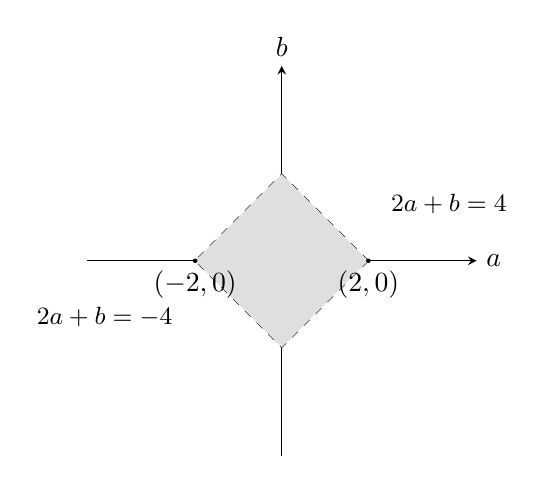
\begin{tikzpicture}[scale=0.55, >=stealth]
  \draw[->] (-4.5,0) -- (4.5,0) node[right] {$a$};
  \draw[->] (0,-4.5) -- (0,4.5) node[above] {$b$};
  \draw[dashed] (2,0) -- (0,2) -- (-2,0) -- (0,-2) -- cycle;
  \fill[gray!25] (2,0) -- (0,2) -- (-2,0) -- (0,-2) -- cycle;
  \fill (2,0) circle (1.5pt) node[below] {$(2,0)$};
  \fill (-2,0) circle (1.5pt) node[below] {$(-2,0)$};
  \node[right] at (2.3,1.3) {\small$2a+b=4$};
  \node[left] at (-2.3,-1.3) {\small$2a+b=-4$};
\end{tikzpicture}
\end{center}
（境界を含む正方形が①の表す領域。直線$2a+b=\pm4$との交点は頂点$(\pm2,0)$のみ。）
\end{proof}

\bigskip
\noindent\textbf{[解2]（全て力ずくに行く）}

\begin{proof}[解2]
$a=0$での成立は明らかだから，以下対称性から$a>0$とする。
\[
g(x)=a\left(x+\frac{b}{2a}\right)^2-\frac{b^2}{4a}
\]
であり，区間内での最大最小値は以下のようになる。
\begin{center}
\begin{tabular}{c|c|c|c}
 & ⑦ $-1\le-\dfrac{b}{2a}\le0$ & ⑦ $0\le-\dfrac{b}{2a}\le1$ & ⑦ otherwise \\
\hline
$\max g$ & $g(1)=a+b$ & $g(-1)=-a+b$ & $a\pm b$のうち小さくない方 \\
\hline
$\min g$ & $g\left(-\dfrac{b}{2a}\right)=-\dfrac{b^2}{4a}$ & $g\left(-\dfrac{b}{2a}\right)=-\dfrac{b^2}{4a}$ & $a\pm b$のうち大きくない方
\end{tabular}
\end{center}
⑦⑦の対称性から，⑦，⑦のみかんがえる。

\textbf{⑦の時}

$a>0$から，$0\le b\le2a$である。これと$\left|a+b+\dfrac{b^2}{4a}\right|\le1\ \therefore\ a+b+\dfrac{b^2}{4a}\le1$から，
\[
b^2+4ab+4a^2-8a\le0
\]
\[
0\le b\le-2a+2\sqrt{2a}
\]
だから，これも図示して右上図斜線部（境界含む）だから，$2a+b=k$との交点から，
\[
0\le2a+b\le4
\]
右の等号成立は$(a,b)=(2,0)$の時。したがって⑦の時も$(a,b)=(2,0)$で$2a+b=4$となる。

\textbf{⑦の時}

軸の条件から，
\[
-\frac{b}{2a}\le-1 \ \text{or}\ 1\le-\frac{b}{2a}
\]
$a>0$から
\[
2a\le b \ \text{or}\ b\le-2a \quad\cdots\text{①}
\]
である。又，値域の幅の条件から
\[
-2\le\bigl|(a+b)-(a-b)\bigr|\le2, \qquad -1\le b\le1 \quad\cdots\text{②}
\]
である。①②を図示して右図斜線部（境界は$a=0$のみ含まず）。したがって，これと$2a+b=k$の交点をかんがえて，
\[
-1<2a+b\le2
\]
だから$|2a+b|<4$

以上から，$|2a+b|\le4$は成立し，等号成立は対称性から$(a,b)=(\pm2,0)$の時。（以下略）
\end{proof}

\newpage

\section*{第3問}

\begin{proof}[解]
$A: x^2+y^2=r^2$，$B: y=\cos\left(\sqrt{\dfrac{\pi}{2}}x\right)$とおく。$A$と$B$の共有点の数は$y$を消した
\[
x^2+\cos^2\left(\sqrt{\frac{\pi}{2}}x\right)=r^2 \quad\cdots\text{①}
\]
の解の数に等しい。この左辺を$f(x)$とおく。$f(x)$は偶関数だから，$x\ge0$でかんがえる。
\[
f'(x)=2x+2\cos\left(\sqrt{\frac{\pi}{2}}x\right)\left(-\sqrt{\frac{\pi}{2}}\sin\left(\sqrt{\frac{\pi}{2}}x\right)\right)=2x-\sqrt{\frac{\pi}{2}}\sin\left(\sqrt{2\pi}x\right)
\]
より，
\[
f'(x)\ge0 \iff 2x\ge\sqrt{\frac{\pi}{2}}\sin\left(\sqrt{2\pi}x\right)
\]
だから左図から下表をうる。
\begin{center}
\begin{tabular}{c|ccccc}
$x$ & $0$ & & $\frac12\sqrt{\frac{\pi}{2}}$ & & $+\infty$ \\
\hline
$f'$ & & $-$ & $0$ & $+$ & \\
\hline
$f$ & $1$ & $\searrow$ & & $\nearrow$ & $+\infty$
\end{tabular}
\end{center}
したがって，グラフは右上図よって解は
\[
\begin{cases}
0<r^2<\dfrac{\pi}{8}+\dfrac12\ \text{の時} & 0\text{個} \\
r^2=\dfrac{\pi}{8}+\dfrac12 & 2\text{個} \\
\dfrac{\pi}{8}+\dfrac12<r^2<1 & 4\text{個} \\
r^2=1 & 3\text{個} \\
1<r^2 & 2\text{個}
\end{cases}
\]
だから
\[
N(r)=
\begin{cases}
0 & \left(0<r<\sqrt{\dfrac{\pi}{8}+\dfrac12}\right) \\
2 & \left(r=\sqrt{\dfrac{\pi}{8}+\dfrac12},\ 1<r\right) \\
3 & (r=1) \\
4 & \left(\sqrt{\dfrac{\pi}{8}+\dfrac12}<r<1\right)
\end{cases}
\]
\end{proof}

\newpage

\section*{第4問}

\begin{proof}[解]
$C: x^2+y^2=1$，$D: (x-4)^2+y^2=4$。時刻$t$での$P,Q$の座標は
\[
P(\cos2t,\sin2t), \qquad Q(4+2\cos t,2\sin t)
\]
とおける。以下$c=\cos t,\ s=\sin t$とおく。
\[
\overline{PQ}^2=(\cos2t-2\cos t-4)^2+(\sin2t-2\sin t)^2
\]
\[
=(\cos^22t+\sin^22t)+\left\{(2c+4)^2+4s^2\right\}-2(2c+4)\cos2t-4s\sin2t
\]
\[
=1+(4+16+16c)-4(c+2\cos2t)
\]
\[
=21+16c-4c-16c^2+8
\]
\[
=-16c^2+12c+29
\]
\[
=-16\left(c-\frac38\right)^2+29+\frac94
\]
から，$-1\le c\le1$とあわせて，

\textbf{$1^\circ$ maxについて}

$c=\dfrac38$で$\max\overline{PQ}=\dfrac{5\sqrt5}{2}$，この時$P\left(-\dfrac{23}{32},\pm\dfrac{3\sqrt{55}}{32}\right)$，$Q\left(\dfrac{19}{4},\pm\dfrac{\sqrt{55}}{4}\right)$（複号同順）

\textbf{$2^\circ$ minについて}

$c=-1$で$\min\overline{PQ}=1$，この時$P(1,0)$，$Q(2,0)$

である。
\end{proof}

\newpage

\section*{第5問}

\begin{proof}[解]
\[
\frac{{}_{3n}C_n}{{}_{2n}C_n}=\frac{(3n)!}{n!(2n)!}\cdot\frac{n!n!}{(2n)!}=\frac{(3n)!\,n!}{(2n)!(2n)!}\equiv f(n)
\]
とおく。$f(n)>0$より，$g(n)=\log f(n)^{\frac1n}$とおくと
\[
g(n)=\frac1n\left(\sum_{k=2n+1}^{3n}\log\frac{k}{n}-\sum_{k=n+1}^{2n}\log\frac{k}{n}\right) \quad\cdots\text{①}
\]
である。ここで
\[
\frac1n\sum_{k=n+1}^{2n}\log\frac{k}{n}\longrightarrow\int_1^2\log x\,dx=2(\log2+1)-1
\]
\[
\frac1n\sum_{k=2n+1}^{3n}\log\frac{k}{n}\longrightarrow\int_2^3\log x\,dx=3(\log3+1)-2(\log2+1)
\]
だから，①より
\[
g(n)\longrightarrow3\log3+4-4\log2-4=3\log3-4\log2=\log\frac{27}{16}
\]
以上から，
\[
\lim_{n\to\infty}\left(\frac{{}_{3n}C_n}{{}_{2n}C_n}\right)^{\frac1n}=\frac{27}{16}
\]
\end{proof}

\end{document}
